\documentclass[12pt, a4paper]{article}

\usepackage[utf8]{inputenc}
\usepackage[russian]{babel}
\parindent 0pt
\parskip 8pt
\usepackage{amsmath}
\usepackage{amssymb}
\usepackage{array}
\usepackage[left=2.3cm, right=2.3cm, top=2.7cm, bottom=2.7cm, bindingoffset=0cm]{geometry} % headheight=0pt,
\usepackage{hyperref}
\usepackage{graphicx}
\usepackage{multicol}
\usepackage{fancyhdr} 
\usepackage{extramarks}

\usepackage[usenames,dvipsnames]{color}
\usepackage{titlesec}
\usepackage[normalem]{ulem}
\usepackage{tikz}
\definecolor{grey}{RGB}{128,128,128}

\pagestyle{fancy}
\fancyhf{}
\lhead{Матан}
\chead{Теормин}
\rhead{\thepage}
\lfoot{}
\cfoot{}
\rfoot{\today}
\renewcommand\headrulewidth{0.4pt}
\renewcommand\footrulewidth{0.4pt}

\titlespacing*{\section}{0pt}{5pt}{0pt}
\titlespacing*{\subsection}{0pt}{5pt}{0pt}
\titlespacing*{\subsubsection}{0pt}{5pt}{0pt}

\begin{document} 
\section{Упорядоченная пара; декартово произведение; операции над множествами}
	\textbf{Упорядоченная пара} - двухэлементное семейство, где множеством индексов является $\{1, 2\}$. При этом в обозначении упорядоченной пары $(a,b)$ считается, что на первом месте стоит элемент, занумерованный индексом $1$, а на втором - индексом $2$. Равенство пар $(a, b)$, $(c, d)$ означает, что $a = b$ и $c = d$.\\
	\textbf{Декартовым} или \textbf{прямым произведением} множеств X и Y называется множество всех упорядоченных пар, таких что первый элемент пары принадлежит $X$ а второй - $Y$.\\
	$X*Y = \{(x, y) : x \in X, y \in Y\}$\\
	\textbf{Операции над множествами:}
	\begin{enumerate}
		\item Пусть $\{X_\alpha _\in _A \}$ - семейство множеств. \textit{Пересечением} семейства $\{X_\alpha _\in _A\}$ назывется множество всех элементов, которые принадлжат каждому из множеств $X_\alpha$:
		$$\bigcap\limits_{\alpha \in A}^{} X_\alpha = \{x : \forall \alpha \in A x \in X_\alpha \}$$
		\item Пусть $\{X_\alpha _\in _A \}$ - семейство множеств. \textit{Объединением} семейства $\{X_\alpha _\in _A\}$ назывется множество всех элементов, которые принадлжат хотя бы одному из множеств $X_\alpha$:
		$$\bigcup\limits_{\alpha \in A}^{} X_\alpha = \{x : \exists \alpha \in A x \in X_\alpha \}$$
		\item \textbf{Разностью} множеств $X$ и $Y$ назывется множество всех элементов, которые принадлежат $X$, но не принадлежат $Y$:
		$$X \backslash Y = \{x : x \in X, x \notin Y \}$$
	\end{enumerate}
\section{Расширенное множество вещественных чисел, операции и порядок в нем}
\begin{figure}[h]
    \centering
    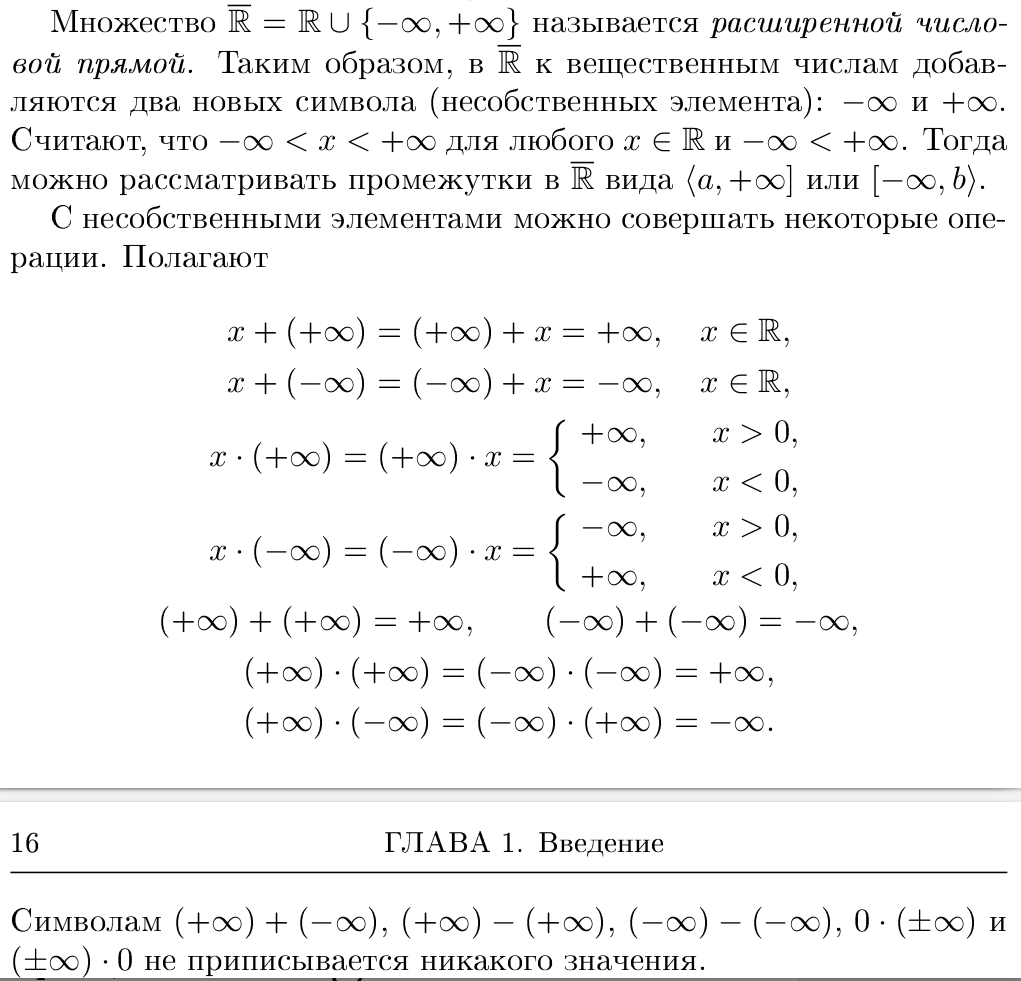
\includegraphics[width=0.8\linewidth]{imagesMin/2.png}
\end{figure}
\section{Подмножество в R, ограниченное сверху}
\begin{figure}[h]
    \centering
    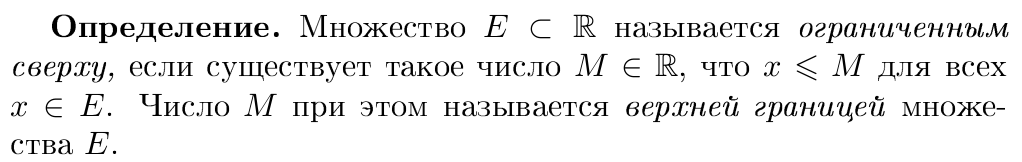
\includegraphics[width=0.8\linewidth]{imagesMin/3.png}
\end{figure}
\section{Максимальный элемент множества}
\begin{figure}[h]
    \centering
    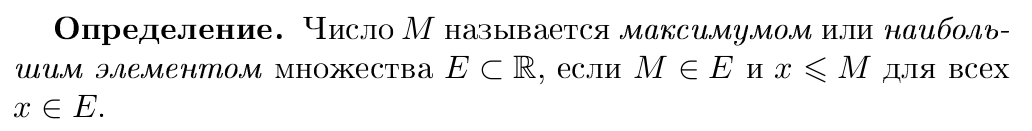
\includegraphics[width=0.8\linewidth]{imagesMin/4.png}
\end{figure}
\end{document}